\documentclass[10pt,journal]{IEEEtran}

\usepackage[scale=0.8]{geometry}
\usepackage{graphicx}

% This centers the captions
\makeatletter
\long\def\@makecaption#1#2{\ifx\@captype\@IEEEtablestring
\footnotesize\begin{center}{\normalfont\footnotesize #1}
{\normalfont\footnotesize\scshape #2}\end{center}
\@IEEEtablecaptionsepspace
\else
\@IEEEfigurecaptionsepspace
\setbox\@tempboxa\hbox{\normalfont\footnotesize {#1.}~~ #2}
\ifdim \wd\@tempboxa >\hsize
\setbox\@tempboxa\hbox{\normalfont\footnotesize {#1.}~~ }
\parbox[t]{\hsize}{\normalfont\footnotesize \noindent\unhbox\@tempboxa#2}
\else
\hbox to\hsize{\normalfont\footnotesize\hfil\box\@tempboxa\hfil}\fi\fi}
\makeatother

\title{Design and implementation of the $sin$ function for an 8-bit MIPS processor}
\author{Dominik Laskowski, Payom Meshgin, Daniel Ranga, Ming Yang}

\begin{document}
\maketitle

\section{Motivation / Background}
Hardware acceleration of transcendental functions is crucial for real-time systems
performing computationally intensive tasks like computer graphics and audio processing.
The x87 floating-point unit in the IA-32 architecture supports instructions like \texttt{fsin}
and \texttt{fsincos}. Likewise, graphics processing units and digital signal processors
provide dedicated logic for trigonometric operations.

Lookup tables based on ROMs and PLAs are the most common approach for implementing $sin$
in hardware. They are often coupled with approximation techniques like interpolation to
achieve adequate precision while reducing transistor count. An alternative method that
offers better precision at the expense of speed is the Taylor series expansion. Finally,
the CORDIC (for Coordinate Rotation Digital Computer) algorithm is desirable in embedded
systems without a multiplier, since it only requires adders, shifters and lookup tables.
In this report, we investigate the design and implementation of a $sin$ functional block for
an 8-bit MIPS processor, using the first two aforementioned approaches.

In practice, $sin$ blocks usually operate on 32-bit IEEE 754 floating-point numbers. However,
since the MIPS core has 8-bit registers and integer operations only, we opted for a custom encoding
scheme based on binary scaling. The assumed domain and image is $[0, \frac{\pi}{2}]$ and $[0, 1]$,
respectively. These ranges are discretized to an integer between $0$ and $255$.

\section{Design Implementation}
\subsection{Lookup Table Implementation}
The $sin$ lookup table is a NOR-NOR PLA with 8-bit input and output. The design process for this
implementation was straightforward. The decimal and binary representations of the 256 angles and
$sin$ results were calculated in an Excel spreadsheet and exported to a CSV file. A simple Python
script was written to convert the CSV file into a Verilog \texttt{casez} statement. The schematic
and layout, shown in Figure \ref{lut}, were obtained from the PLA generator and tweaked in Electric
to pass DRC. Figure \ref{mips_lut} is the final layout after the lookup table was mirrored vertically
and wired up to the datapath.

\begin{figure}[h]
\centering
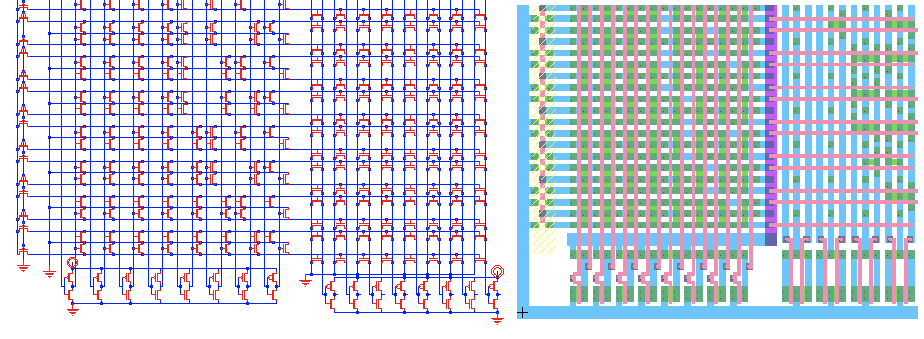
\includegraphics[width=3in]{lut.png}
\caption{Schematic and layout of the lookup table}
\label{lut}
\end{figure}

\begin{figure}[h]
\centering
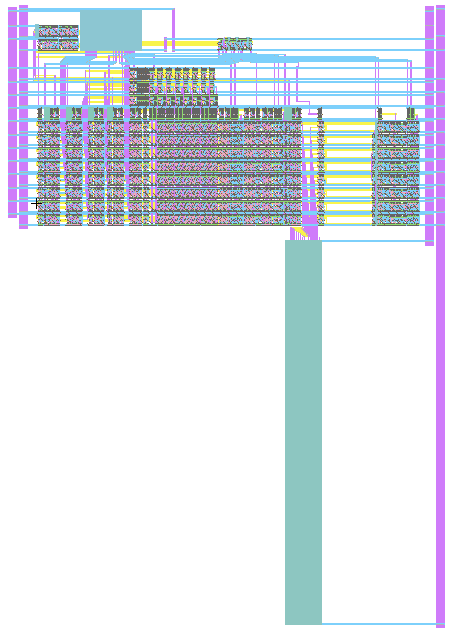
\includegraphics[width=3in]{mips_lut.png}
\caption{Layout of MIPS core with lookup table}
\label{mips_lut}
\end{figure}

\subsection{Taylor expansion design}
\begin{equation}
\label{sin-taylor}
sin(x) = x - \frac{x^3}{3!} + \frac{x^5}{5!}+ O(x^7)
\end{equation}

\begin{figure}[h]
\centering
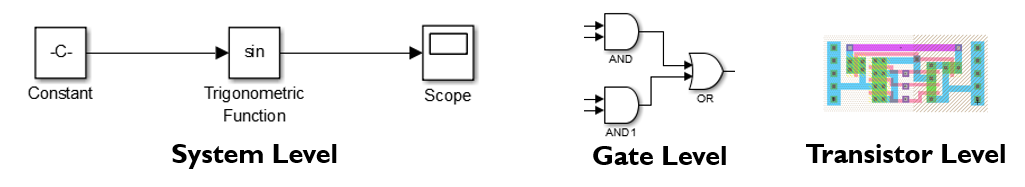
\includegraphics[width=3in]{design_methodology.png}
\caption{Circuit Design Methodology}
\label{design_methodology}
\end{figure}

The formula written in equation \ref{sin-taylor} is a three-term expansion of Taylor series for $sin(x)$. In this project, we implemented a combinational logic circuit based on this equation to evaluate the $sin$ function. The reason for choosing that is related to the goal of this project, which is to have a $sin$ function generator with an accuracy that is comparable to the LUT solution, and Taylor series does provide an adjustable accuracy, based on the number of terms included the evaluation.

During the design phase of this circuit, as shown in Fig.\ref{design_methodology}, a top-to-down design approach is followed to implement system-level, gate-level and transistor level design of the entire system. More specifically, due to the fact that the same interface is used for circuit design and simulation in Simulink, circuit design becomes much more efficient than the case that it is designed in Electric and then get verified in ModelSim. Therefore, the system-level and gate level design and simulation are both implemented in Simulink, and then they are directly translated into Electric to implement the transistor-level design after the gate-level design functionality has been verified. 

\begin{figure}[h]
\centering
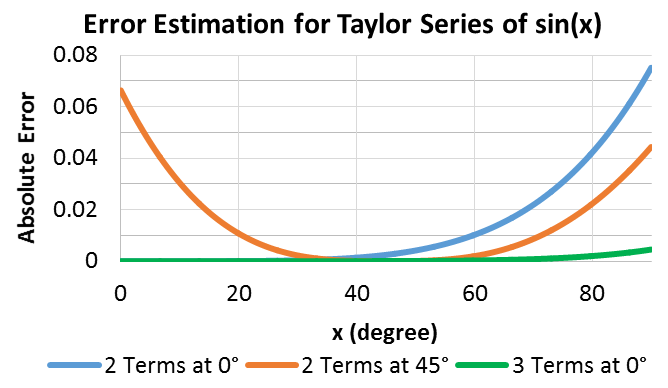
\includegraphics[width=3in]{error-estimation.png}
\caption{Absolute approximation error with different Taylor series}
\label{error-estimation}
\end{figure}

At the beginning of the project, an error estimation process is conducted to help us identify the target of this design so that the corresponding circuit can be build up based on specific design requirements. Fig.\ref{error-estimation} demonstrates the absolute approximation error caused by applying Taylor series with different conditions. Since the design is required to have similar accuracy as the LUT implementation (error ≤0.2\%), we decided to use three terms Taylor series and expand it respect to zero so that the estimation error is ensured to be smaller than 0.5\%.

\begin{figure}[h]
\centering
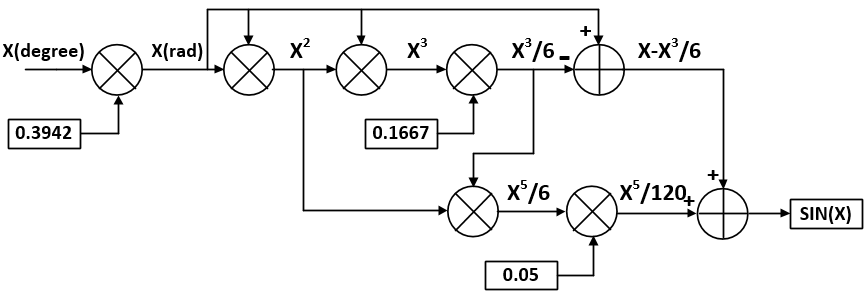
\includegraphics[width=3in]{finalized_design.png}
\caption{Finalized system-level design of Taylor series implementation}
\label{finalized_design}
\end{figure}

Fig.\ref{finalized_design} illustrates the finalized system-level implementation of Taylor series implementation and several optimizations have been made at this level. First of all, some of the generated numbers, such like $x^2$ and $x^3/6$, can be reused in this algorithm to reduce the complexity of the circuit. Second, division can be carried out by multipliers since the dividend is always larger than one. The cost can be further reduced by shifting operation if the dividend contains a factor of 2. To make the design consistent with our loop-up table implementation, we were about to encode all the fixed point numbers by shifting 8 bits in our system. However, it turns out that this will lead to an error if the input value becomes larger than 1 in radians degrees). Therefore, as demonstrated in the figure, a multiplier is placed in the front end of the entire circuit so that the input value can be encoded by shifting 6 bits to the right, and the fixed point precision has to be compromised by 2 bits.

\begin{figure}[h]
\centering
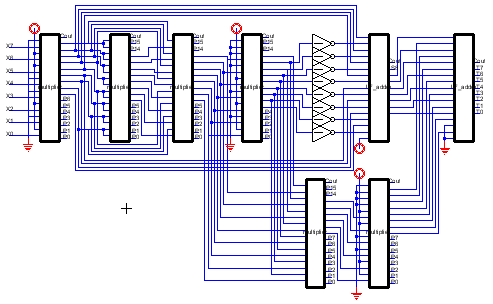
\includegraphics[width=3in]{finalized_gate_design.png}
\caption{Finalized gate-level design of Taylor series implementation}
\label{finalized_gate_design}
\end{figure}

In schematic design, based on the information provided in the textbook, the 8-bits Ladner-Fischer adder and carry-save adder design are performed in the multiplier design to effectively reduce the propagation delay on the critical path. Mirrored version of carry-save adder is also used to improve its shape during the layout process so that it will be in an organized rectangular form. Fig.\ref{finalized_gate_design} shows the finalized gate-level schematic design for the overall system in Electric.

\begin{figure}[h]
\centering
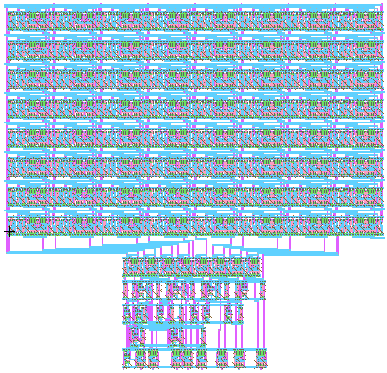
\includegraphics[width=2in]{finalized_transistor_design.png}
\caption{Finalized transistor-level layout design of multiplier}
\label{finalized_transistor_design}
\end{figure}

The transistor-level implementation is performed based on the validated schematic design demonstrated in the previous section. Fig.\ref{finalized_transistor_design} illustrates the layout design of the 8-bits multiplier. The carry-save adder section is well organized in a rectangular shape and a LF adder is placed on the bottom to sum up each carry bit. The entire system is organized in a similar way, and because of the correct methodology practiced in this design, the simulation for the system was successful for the first trial.

\subsection{Modification to MIPS processor}
+A conservative method was used to connect the generated functional block to the available MIPS core. For the purpose of integration the functional blocks are 8-bit input, 8-bit output black boxes which act as an extended arithmetic operation. As such, the $sin$ operation  is treated as an R-type instruction , operating in parallel with the present ALU (for which the second source register is ignored). The assigned function code to $sin$ is 101111. This approach requires modification to the ALU decoder while keeping MIPS state controller intact. The ALU decoder is extended by an other output : \texttt{$ALUctrl[3] =  ALUop[1] \cdot \overline{funct[0] \cdot funct[2] \cdot funct[3]}$}. \texttt{ALUctrl[3]} is used as a select signal to a 2:1 wordslice multiplexer, choosing as output either the result generated by the ALU, when performing an ALU task, or the result from the $sin$ functional block. While the equation for \texttt{ALUctrl[3]} may not be optimized given the available signals within the ALU decoder the extra logic is neither limiting in the context of local routing nor in the context of total area. Finally, the ALU and circuits to the right of it have to be moved to the right to allow insertion of the mux wordslice and permit routing of two 8-bit busses (\texttt{srcA} and \texttt{result}) as the implementation of the $sin$ block wasn't possible within the row constraints set by the datapath.

\section{Validation}
	
	\subsection{Look-up table design}
	\subsection{Taylor expansion design}
	\subsection{Modification to MIPS processor}

\section{Results \& Evaluation}
The two implementations of the design were evaluated using the following three metrics:
\begin{itemize}
\item Accuracy (Error between the output of functional block and the theoretical evaluation of the sine function)
\item Size (Number of transistors in the layout of the functional block)
\item Scalability (How the complexity of the design scales as the bit-width of the signals increase)
\end{itemize}

\subsection{Results \& Accuracy}
The accuracy of the evaluation is very important for functional blocks such as our sine block. Naturally, the evaluation of the block at any input is designed to match the theoretical result of the sine function at the discrete points defining the input domain of the block. Fig. \ref{results} shows how closely both implementations of the sine block follow the theoretical value of the function over the entire input domain.
\begin{figure}[h]
\centering
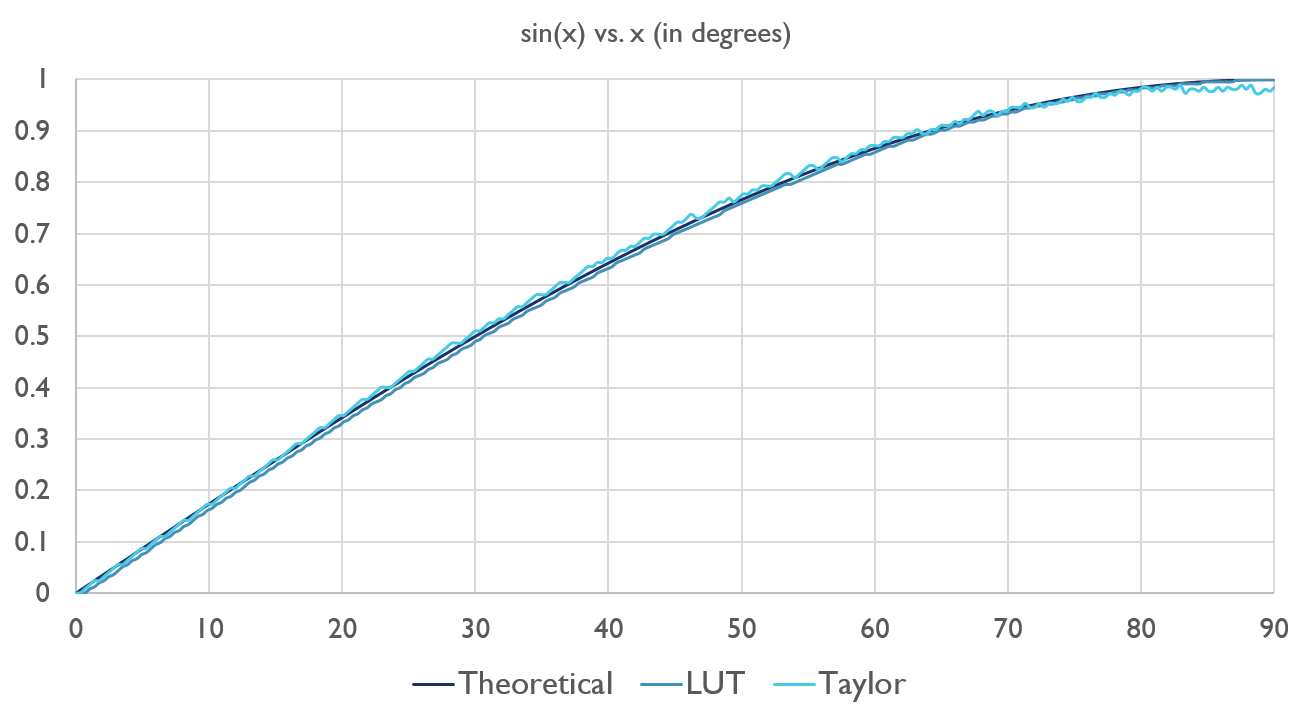
\includegraphics[width=3in]{results.png}
\caption{Evaluations of the sine function using both implementations and the theoretical value}
\label{results}
\end{figure}

In Fig.\ref{errors}, a more precise view of the accuracy is shown. From the plot, it is evident the accuracy of the lookup table based implementation is extremely accurate. This is, of course, not a surprise, since the look-up table is designed such that for a given input, the block takes as output the closest value to the theoretical sine function. Hence, the absolute error for the LUT design never exceeds the error due to quantization, which for this digital design is equal to $2^{-9} \approx 0.002$.

As for the Taylor expansion design, the accuracy is greater than that of the LUT implementation of the sine block. This behaviour is explained by the loss of precision incurred while evaluating the Taylor series terms. The dominant error term is hence $2^{-7}$, due to the reduction of fixed point precision to 6 bits. In addition, some of the error, especially near the end of the input range, is caused by the Taylor series expansion itself, namely the fact that only its three most dominant terms are computed.

\begin{figure}[h]
\centering
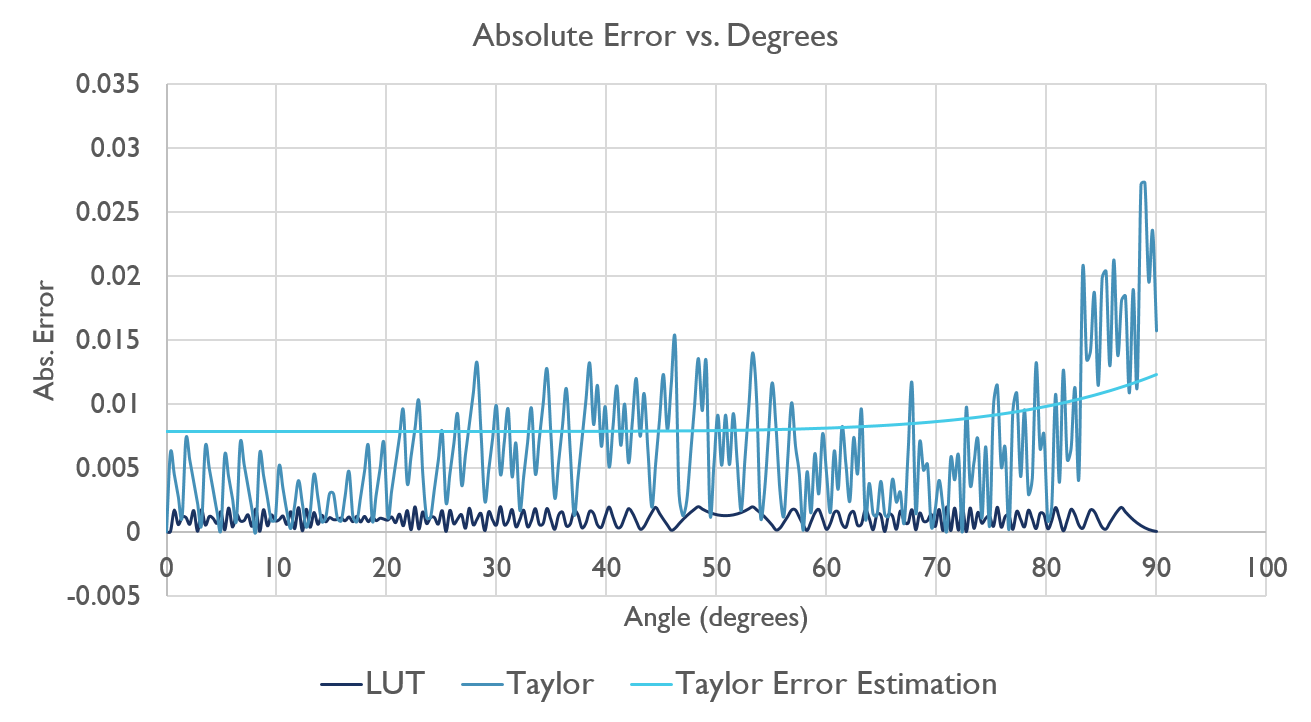
\includegraphics[width=3in]{errors.png}
\caption{Plot of the absolute error for each evaluation of either implementation of the sine block}
\label{errors}
\end{figure}

\subsection{Size}
The area of both implementations of the block were measured as follows:
\begin{itemize}
	\item LUT: $3200 \lambda \cdot 300 \lambda = 0.96 \cdot 10^6 \lambda^2$
	\item Taylor: $7000 \lambda \cdot 4700\lambda = 32.9 \cdot 10^6 \lambda^2$ %TODO 
\end{itemize}
The lookup table design is significantly smaller than the Taylor expansion design, both in terms of area as well as the number of transistors. Indeed, the Taylor implementation of the functional block dwarfs the entire MIPS core in size, as seen in the image of the integrated design (Fig.\ref{taylor_global}).

\begin{figure}[h]
\centering
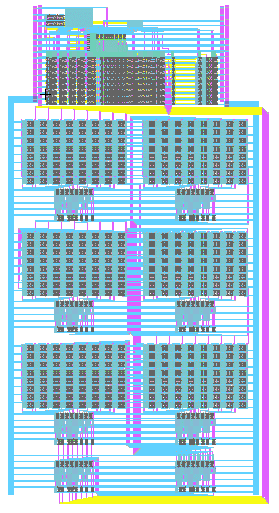
\includegraphics[width=1in]{taylor_global.png}
\caption{Overall layout design of the integrated system including the Taylor expansion implementation and the MIPS core.}
\label{taylor_global}
\end{figure}

\subsection{Scalability}
The scalability of each implementation differs. Given $n$ as the bit-width of the operand ($n = 8$ bits in this case), the LUT based implementation scales quadratically as the precision of the operation increases, so the complexity of the design is on the order $O(n^2)$. The Taylor expansion based design, however scales linearly, which leads to a smaller difference between the sizes of the two implementations.

\section{Possible improvements}
There are a number of improvements to the current design that would improve the functionality of the sine block. Most importantly, a linear interpolation could be employed for the LUT design, which would greatly reduce area and number of transistors at the expense of a slightly larger error. This modification, involving the use of an additional $(n)$-bit wide adder, is essential for larger-precision environments (32-bit, 64-bit).

Another improvement would be to extend the functionality of the block. For example, the sine block could be extended such that the input angle can be within the range 0 to 180 or the entire possible range of angles. Moreover, other trigonometric functions could be implemented with minor modifications to the current design, such as the cosine (using an adder) and tangent (using a divider) functions.

Finally, the MIPS core can also be extended to improve the performance of the functional block. For instance, the MIPS core could be modified to enable multicycle evaluation, using the ALU to compute all each addition and sum need to evaluate a Taylor expansion. This modification  leads to greater savings in area and in the number of transistors.

If the LUT can be rotated $90^{\circ}$ the LUT integrated MIPS core would be small enough vertically to package (horizontally, the package may require the addition of pins or an increase in pin spacing). While the system does work, it is highly unlikely the layout is can be manufactured due to a significant amount of long parallel wires, especially tying the functional block to the the datapath. Additionally, there was no attempt made to scale the gates driving these long routing wires.

As implemented the MIPS core could accept many more functional blocks similar to $sin$. Each function would require it's own function code, an input on the wordslice mux and the ALU control codification would have to be extended.

Finally, while the functional implementation operates on an 8-bit number it is possible to extend functionality to 16 bits as both \texttt{srcA} and \texttt{srcB} are available as inputs to the ALU. It would also be possible to extend the output to 16 bits however this would require modifying the core state machine as it would require two write cycles instead to the single cycle R-type operations allow.

\section{Conclusion}
In conclusion, two methods to compute the $sin$ function have been implemented, integrated into the MIPS core and functionally validated, one using a look-up table PLA another using a mathematical Taylor series expansion. The block's operation relies on a custom input and output encoding which requires the programmer to validate that the input data is as intended and to perform post-processing operations on the output as required. For an 8-bit wide implementation the LUT implementation performs best while maintaining the smallest area however as bus width increases the Taylor series implementation becomes more advantageous area-wise. Still, in that particular case, an lookup table based model with linear interpolation is likely superior to any Taylor series expansion.

\end{document}
